\addcontentsline{toc}{section}{Audio Casette (3)}
\section*{Audio Casette}

\subsection*{Problem}

Find the thickness $h$ and density $\rho$ of the tape of an audio casette.
The coil cores have radius $r = 11.0\text{ mm}$ and
the mass of the whole casette is $M = 40\text{ g}$

Equipment given: audio casette, pencil, calipers.

\subsection*{Solution}

In order to measure something,
we first have to transport all the tape to one of the coils (namely first).
Then we can do $N$ rotations of the second coil and measure
the radius ratio of the coils and the position of the center of mass.

The radius of the coils is measured as follows:
you turn one of the coils by some angle
(can be measured using the teeth of the coil),
and follow the rotation of the other coil.
The ratio of the angles is the ratio of radii.
The process should be reversed before continuing.
The mass center position can be found
by just pushing the casette of something's edge
and measure the position using the calipers.
It's better to use the calipers itself as the "something"
for better precision.

\newcommand{\inlfrac}[2]{+#1/#2}
The measurements are as follows
\begin{center}
    \begin{tabular}{ c | c | c | c | c}
    N   & $\alpha_1 [2\pi]$ & $\alpha_2 [2\pi]$ & $r_1 / r_2$ & $x_c[\text{ m}]$\\
    \hline
    0   &   5       & $2\inlfrac{1}{6}   $ & 2.31 & 0.0935   \\
    50  &   3       & $1\inlfrac{5}{12}  $ & 2.12 & 0.0932   \\
    100 &   3       & $1\inlfrac{13}{24} $ & 1.95 & 0.0928   \\
    150 &   3       & $1\inlfrac{2}{3}   $ & 1.80 & 0.0924   \\
    200 &   2       & $1\inlfrac{1}{4}   $ & 1.60 & 0.0920   \\
    250 &   4       & $2\inlfrac{3}{4}   $ & 1.45 & 0.0914   \\
    300 &   2       & $1\inlfrac{1}{2}   $ & 1.33 & 0.0909   \\
    350 &   5       & $4\inlfrac{1}{12}  $ & 1.22 & 0.0902   \\
    400 &   4       & $3\inlfrac{7}{12}  $ & 1.12 & 0.0894   \\
    450 &   2       & $1\inlfrac{11}{12} $ & 1.04 & 0.0887   \\
    500 &   4       & $4\inlfrac{1}{4}   $ & 0.94 & 0.0880   \\
    550 &   4       & $4\inlfrac{3}{4}   $ & 0.84 & 0.0874   \\
    600 &   3       & $3\inlfrac{11}{12} $ & 0.77 & 0.0867   \\
    650 &   3       & $4\inlfrac{5}{12}  $ & 0.68 & 0.0857   \\
    700 &   3       & $5\inlfrac{1}{12}  $ & 0.59 & 0.0848   \\
    750 &   1       & $2               $ & 0.50 & 0.0840   \\
    800 &   1       & $2\inlfrac{1}{2}   $ & 0.40 & 0.0831   
    \end{tabular}
\end{center}
we will later see,
that the $0$ point for $x_c$ measurement doesn't matter.

Theoretically we can write the radius ratio as
\begin{equation}
    \frac{r_1}{r_2} = k = \frac{\sqrt{(r + h N_0)^2 + r^2 - (r + h N)^2}}{r + h N}
\end{equation}
as the side surface of the tape $\propto r_1^2 + r_2^2$ conserves.
Here $N_0$ is full number of rotations.
This can be linearized to
\begin{equation}
    \sqrt{1+k^2} = -\frac{h}{r} \sqrt{1+k^2} N + \sqrt{\inb({1+ N_0 h / r})^2 + 1}
\end{equation}
and by plotting $\sqrt{1+k^2}$ on $N \sqrt{1+k^2}$ (\reff{S-1}) one can get
$h = r \cdot 1.7\cdot10^{-3} = 1.9 \cdot 10^{-5} \text{ m}$.

\begin{figure}
    \centering

    \begin{subfigure}[l]{.49\textwidth}
        \centering
        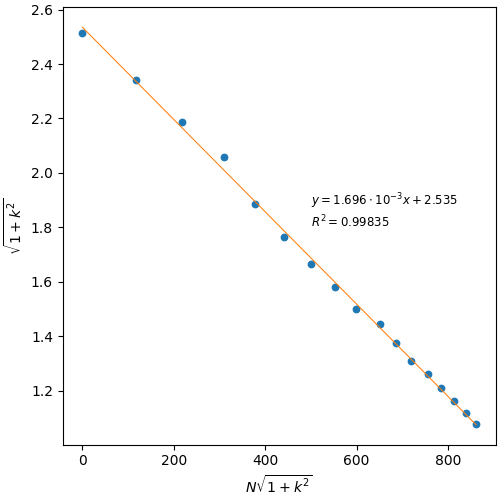
\includegraphics[width = \textwidth]{S-1}
        \caption{}
        \labelf{S-1}
    \end{subfigure}
    \hfill
    \begin{subfigure}[l]{.49\textwidth}
        \centering
        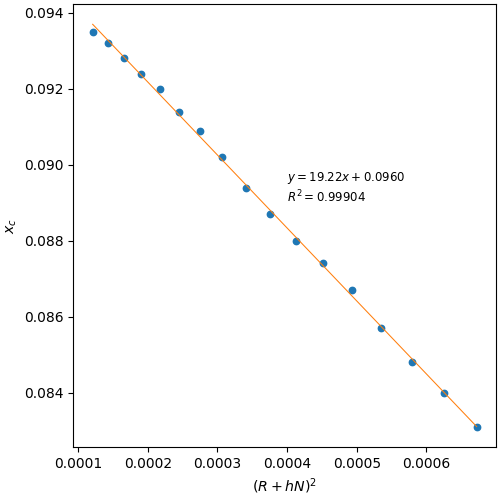
\includegraphics[width = \textwidth]{S-2}
        \caption{}
        \labelf{S-2}
    \end{subfigure}
    
    \caption{}
    \labelf{S-1-2}
    \vspace{-.5cm}
\end{figure}

The position of the center of mass is theoretically given as
\begin{equation}
    x_c = \frac{m_* x_* - \rho \pi w h l (r + h N)^2 }{M}
\end{equation}
where $w$ is the width of the tape and
$l$ is the distance between coil centers,
which can be measured directly.
$w = 3.8 \cdot 10^{-3}\text{ m}$, $l = 4.23 \cdot 10^{-2}\text{ m}$.
$m_*$ and $x_*$ are some arbitrary units
which include the casette box and some residual terms from the calculation.

So by plotting $x_c$ on $(r + h N)^2$ \reff{S-2} we get
$\rho = M / \pi w l \cdot 19.2 \text{ m}^{-1} = 1.5 \cdot 10^3 \text{ kg} / \text{m}^3$.
